\documentclass[dvipsnames, svgnames, x11names, 11pt]{article}

\setlength{\columnsep}{20pt}

\usepackage[paper=a4paper, top=2cm, bottom=3cm, right=2.6cm, left=2.6cm]{geometry}

\usepackage{xcolor}
% URLs and hyperlinks ------------------------------
\usepackage{hyperref}
\hypersetup{
    colorlinks=true,
    linkcolor=DarkBlue,
    filecolor=magenta,
    urlcolor=blue,
}
\usepackage{xurl}
%---------------------------------------------------

\usepackage{graphicx}
\usepackage{xepersian}
\settextfont{Yas}

\title{فاز اول پروژه}
\author{
محدثه آخوندی \\
مهدی حق‌وردی \\
سعید رنجبر
}
\date{}

\begin{document}
\maketitle
\tableofcontents

\section{مصاحبه و جمع‌آوری نظرات در ارتباط با مدل اولیه}

\subsection{سوالات}
\begin{itemize}
\item 
به نظر شما چه عواملی باعث گرایش جوانان به مصرف مواد مخدر یا الکل می‌شود؟
\item 
چه راه‌هایی برای افزایش آگاهی در مورد مضرات مصرف مواد مخدر و الکل وجود دارد؟
\item 
آیا به نظر شما آموزش از طریق فضای مجازی می‌تواند موثر باشد؟ چرا؟
\item 
به نظر شما چه نوع فعالیت‌های تفریحی می‌تواند جایگزین رفتارهای پرخطر شود؟
\item 
چه عواملی می‌توانند انگیزه شما را برای یادگیری و تغییر رفتار افزایش دهند؟
\item 
چه انتظاری از شهرداری در ارائه راهکارهای پیشگیری از اعتیاد دارید؟
\end{itemize}

\subsection{پاسخ‌های خلاصه‌سازی شده و حاوی موارد مشترک}
\begin{itemize}
\item 
دلایل گرایش جوانان به مصرف مواد مخدر و الکل

\begin{itemize}
\item 
فشار روانی، استرس، و مشکلات شخصی (مشکلات خانوادگی، بیکاری).
\item 
تقلید از دوستان و کنجکاوی.
\item 
نبود تفریحات مناسب و حمایت خانوادگی.
\end{itemize}

\item 
راه‌های افزایش آگاهی

\begin{itemize}
\item 
برگزاری کارگاه‌های آموزشی در مدارس، دانشگاه‌ها و محیط‌های کاری.
\item 
تولید محتواهای جذاب و علمی در فضای مجازی (ویدیوهای آموزشی، انیمیشن).
\item 
پخش برنامه‌های تلویزیونی و توزیع بروشورهای اطلاع‌رسانی.
\end{itemize}

\item 
تاثیر آموزش در فضای مجازی

\begin{itemize}
\item 
اکثریت معتقدند آموزش‌های مجازی موثر است به شرط تولید محتوای باکیفیت و جذاب.
\item 
برخی تاکید بر ترکیب روش‌های سنتی و مدرن دارند.
\end{itemize}

\item 
جایگزین‌های رفتارهای پرخطر

\begin{itemize}
\item 
ورزش‌های گروهی و انفرادی (فوتبال، پیاده‌روی، یوگا).
\item 
فعالیت‌های هنری و مهارتی (نقاشی، موسیقی، آشپزی).
\item 
برنامه‌های گروهی و سفرهای کوتاه.
\end{itemize}

\item 
عوامل انگیزشی
\begin{itemize}
\item 
مشاهده تغییرات مثبت و پیشرفت‌های ملموس در زندگی.
\item 
تشویق‌های مالی یا معنوی.
\item 
حمایت خانواده و اطرافیان.
\end{itemize}

\item 
انتظارات از شهرداری
\begin{itemize}
\item 
ایجاد فضاهای تفریحی، ورزشی، و فرهنگی رایگان یا با هزینه کم.
\item 
برگزاری رویدادها و کارگاه‌های آموزشی.
\item 
حمایت از مشاوره‌های رایگان روان‌شناسی.
\end{itemize}

\item 
احتمال استفاده از اپلیکیشن
\begin{itemize}
\item 
میانگین احتمال استفاده: حدود 60-70 درصد.
\item 
عوامل موثر بر پذیرش: جذابیت، کارایی، حفظ حریم شخصی.
\end{itemize}

\item 
پیشنهادات برای بهبود پلتفرم

\begin{itemize}
\item 
اضافه کردن داستان‌های موفقیت و مشاوره‌های تخصصی.
\item 
برگزاری رویدادهای آنلاین و آفلاین.
\item 
گیمیفیکیشن و سیستم‌های تشویقی.
\end{itemize}

\item 
پرداخت هزینه برای نسخه پریمیوم

\begin{itemize}
\item 
برخی حاضر به پرداخت هزینه هستند به شرط ارائه خدمات منحصربه‌فرد و کاربردی.
\item 
قیمت مناسب و تفاوت محسوس بین نسخه رایگان و پریمیوم ضروری است.
\end{itemize}

\item 
ویژگی‌های مهم

\begin{itemize}
\item 
حفظ حریم شخصی.
\item 
سهولت استفاده و دسترسی آسان.
\item 
جذابیت بصری و گرافیک حرفه‌ای.
\end{itemize}
\end{itemize}

\section{بررسی و جمع بندی ارزیابیها، نقدها و پیشنهادات دانشجویان}

\subsection{نقاط قوت مدل کسب و کار}
\begin{itemize}
\item 
ارائه خدمات جامع

ترکیب مشاوره، درمان، آموزش، و پشتیبانی مستمر که نیازهای مختلف کاربران را پوشش می‌دهد.

\item 
ایجاد شبکه حمایتی قوی

جامعه‌ای حمایتی برای افراد آسیب‌دیده که از لحاظ روحی و انگیزشی مفید است.

\item 
ارتباط ناشناس با مشاوران

کاربران می‌توانند بدون افشای هویت خود مشاوره بگیرند، که باعث احساس امنیت می‌شود.

\item 
سیستم تشویقی و انگیزشی

استفاده از ابزارهایی مثل توکن برای ایجاد انگیزه و امکان درآمدزایی برای کاربران.

\item 
تمرکز بر آموزش

ارتقای دانش و آگاهی افراد درباره مشکلات و راه‌حل‌ها.

\item 
دسترسی و پشتیبانی دائمی

خدمات 24 ساعته که کاربران را در هر زمان پشتیبانی می‌کند.

\item 
استفاده از کانال‌های متنوع ارتباطی

ایجاد ارتباط آسان و موثر با مشتریان از طریق روش‌های مختلف.

\item 
تمرکز بر نیازهای فردی

برنامه‌ها و خدمات متناسب با نیازهای خاص هر کاربر.
\end{itemize}

\subsection{نقاط ضعف مدل کسب و کار}
\begin{itemize}
\item 
نیاز به نوآوری

خدمات ارائه‌شده به ایده‌های جدید و خلاقانه بیشتری نیاز دارند.

\item 
مشکلات اعتمادسازی

بسیاری از کاربران احساس می‌کنند نیاز به شفافیت و اعتمادسازی بیشتری وجود دارد.

\item 
عدم ارائه راه‌حل‌های عملی

پاسخ‌های مشخص و قابل‌اجرا برای مشکلات کمتر ارائه شده است.

\item 
عدم تمرکز کافی بر پیشگیری

خدمات بیشتر بر درمان متمرکز هستند و به پیشگیری از مشکلات کمتر توجه شده است.

\item 
چالش در همسو کردن جامعه‌های هدف

سختی در یکپارچه‌سازی نیازهای مخاطبان مختلف، مانند افراد آسیب‌دیده و جوانان.

\item 
مشوق‌های ناکافی

نبود پیشنهادات جذاب برای جذب و حفظ کاربران.

\item 
نیاز به بهبود ارتباطات

مشکلاتی در ارتباط دائمی و موثر با کاربران دیده می‌شود.

\item 
فقدان شفافیت در ارزش پیشنهادی

برخی کاربران احساس می‌کنند اهداف و خدمات به اندازه کافی مشخص نشده‌اند.
\end{itemize}

\subsection{میانگین نمرات و امتیازات عددی}
\begin{itemize}
\item 
از ۱ تا ۵ به میزان اهمیت مشکل برای مشتریان امتیاز بدهید.

نمره‌ی متوسط: $4.15$

\item 
با توجه به بخش مشتریان چه امتیازی به ارزش پیشنهادی می دهید؟

نمره‌ی متوسط: $4.08$
\item 

به راه‌حل ارائه شده امتیاز دهید. به راه‌حل ارائه شده امتیاز دهید.

نمره‌ی متوسط: $3.91$
\item 
در کل به مدل کسب و کار  ارائه شده چه امتیاز می دهید؟

نمره‌ی متوسط: $4.13$

\end{itemize}

\section{بررسی و تحلیل عمیق رقبا}

\subsection{فرهنگسرای امید}
\subsubsection{راه‌حل‌ها}
\begin{itemize}
\item 
جلسات بازآفرینی گروهی و حضوری
\end{itemize}

\subsubsection{توضیحات تکمیلی}
\begin{itemize}
\item 
موارد قوت

این جلسات با حضور افراد مختلف است که به صورت هفتگی است. افراد مختلف حضور پیدا میکندد و الهام بخش یکدیگر هستند و به هم انرژی میدهند. جو صمیمی که به وجود می آید بسیار مهم است و همچنین اینکه آنجا افراد با یکدیگر دوست میشوند و به واسطه دوستی ترک اعتیاد راحت تر است.

\item
موارد ضعف

به واسطه حضوری بودن همه افراد از هر جای کشور قاعدتا نمیتوانند بیایند و ممکن است محدودیت فیزیکی نیز داشته باشند. مورد دیگر نیز بعضی از افراد که نمیخواند هویت شان فاش شود نمیتوانند در این جلسات حضور پیدا کنند چراکه افرادی که می آیند مشخص است و نمیشود به صورت ناشناس در این جلسات شرکت کرد.
\end{itemize}


\subsection{کمپ ترک اعتیاد فرمانیه}
\subsubsection{راه‌حل‌ها}
\subsubsection{توضیحات تکمیلی}
\begin{itemize}
\item 
نقاط قوت

این مرکز با متخصصان و امکاناتی که دارد مشخصا میتواند به راحتی اعتماد مراجعه کنندگان را بدست بیارد که به شرح زیر است:

\begin{itemize}
\item 
متخصصان

جناب آقای دکتر علیرضا محمودنژاد مدیریت مجموعه، جناب آقای دکتر علیرضا محتشم الشریعه متخصص روانپزشکی، جناب آقای سعید جلیلی نیکو روانشناس و درمانگر، جناب آقای دکتر کیهان حسنی پزشک عمومی و مسئول فنی

\item
امکانات

منوی غذایی با کیفیت، استخر، باشگاه ورزشی، سرگرمی، جلسات خانواده
\end{itemize}
این شرایط بسیار شرایطی خوبی برای ترک کردن و همچین آگاهی بخشی است و کمک کننده است به ترک معتادان.

\item 
نقاط ضعف

از جمله نقاط ضعفی که میشود اشاره کردن این است که این کمپ خصوصی است و عامه مردم نمیتوانند از آن استفاده کنند و همچنین با توجه به شرایط آن هزینه آن نیز گزاف خواهد بود و همه این ها در کنار هم باعث میشود که تنها افراد خاصی بتوانند از خدمات این کمپ استفاده کنند. مورد بعد حضوری بودن ان است. یعنی صرفا افرادی که برای آن شهر و منطقه هستند میتوانند استفاده کنند ازین شرایط و معتادان شهر های دیگر قابلیت استفاده از ان را ندارند.
\end{itemize}


\subsection{\lr{Sober Grid}}
\subsubsection{راه‌حل‌ها}
\begin{itemize}
\item 
شبکه اجتماعی

\lr{Sober Grid}
یک شبکه اجتماعی برای افرادی است که به دنبال ترک اعتیاد یا حفظ سبک زندگی پس از ترک هستند. این اپلیکیشن امکان تعامل، اشتراک‌گذاری تجربه‌ها، و دریافت حمایت از دیگر کاربران در سراسر دنیا را فراهم می‌کند.

\item 
مشاوره آنلاین

کاربران می‌توانند از روانشناسان و مشاوران ترک اعتیاد به صورت آنلاین مشاوره بگیرند. این ویژگی برای افرادی که به کمک فوری نیاز دارند بسیار کاربردی است.

\item 
تحلیل داده‌ها

اپلیکیشن از داده‌های کاربران (مانند مدت زمان پاکی، تغییرات روحی، و رفتارها) برای ارائه گزارش‌های پیشرفت استفاده می‌کند و این اطلاعات را به شکلی ساده و کاربردی در اختیار آن‌ها قرار می‌دهد.
\end{itemize}

\subsubsection{توضیحات تکمیلی}
\begin{itemize}
\item
نقاط قوت

\begin{itemize}
\item 
جامعه جهانی

یکی از بزرگ‌ترین مزایای \lr{Sober Grid} حضور یک جامعه جهانی از افراد ترک‌کرده است. کاربران می‌توانند از تجربه‌های یکدیگر بهره‌مند شوند و احساس کنند که تنها نیستند.

\item 
رابط کاربری ساده و جذاب

طراحی اپلیکیشن به گونه‌ای است که حتی افراد با کمترین آشنایی با فناوری نیز می‌توانند به راحتی از آن استفاده کنند.

\item 
ویژگی‌های تحلیل داده
\item 
ابزارهای پیشرفته‌ای برای ردیابی و نظارت بر پیشرفت کاربران وجود دارد. این ویژگی می‌تواند برای کاربران انگیزشی باشد تا در مسیر ترک پایدار بمانند.
\end{itemize}

\item
نقاط ضعف
\begin{itemize}
\item 
محتوای آموزشی محدود

اگرچه ویژگی‌های اجتماعی و مشاوره‌ای اپلیکیشن قوی است، اما محتوای آموزشی برای آگاهی‌بخشی و پیشگیری از اعتیاد محدود است.

\item 
هزینه اشتراک

برخی امکانات پیشرفته، مانند مشاوره روانشناسی یا گزارش‌های تخصصی، نیازمند پرداخت هزینه اشتراک است که ممکن است برای همه کاربران مقرون‌به‌صرفه نباشد.

\item 
تمرکز محدود

اپلیکیشن بیشتر بر حفظ سبک زندگی پس از ترک تمرکز دارد و برنامه‌های کمتری برای پیشگیری یا آموزش عمومی ارائه می‌دهد.
\end{itemize}
\end{itemize}

\subsection{\lr{Quit Genius}}
\subsubsection{راه‌حل‌ها}
\begin{itemize}
\item 
درمان شناختی-رفتاری \lr{(CBT)}

\lr{Quit Genius}
از اصول درمان شناختی-رفتاری استفاده می‌کند که بر تغییر الگوهای فکری و رفتاری افراد تمرکز دارد. این رویکرد برای ترک اعتیاد به الکل، مواد مخدر، و حتی سیگار بسیار مؤثر است.

\item 
پشتیبانی با هوش مصنوعی

این اپلیکیشن از چت‌بات‌های هوشمند برای ارائه پشتیبانی فوری و پاسخ به سوالات کاربران استفاده می‌کند. علاوه بر این، مشاوران حرفه‌ای نیز برای راهنمایی‌های تخصصی در دسترس هستند.

\item 
شخصی‌سازی
\lr{Quit Genius}
از هوش مصنوعی برای تحلیل رفتارهای کاربر و ارائه برنامه‌های شخصی‌سازی‌شده استفاده می‌کند. این برنامه‌ها با توجه به نیازها و شرایط خاص هر فرد طراحی می‌شوند.
\end{itemize}

\subsubsection{توضیحات تکمیلی}
\begin{itemize}
\item 
نقاط قوت
\begin{itemize}
\item 
استفاده از علم روانشناسی

طراحی محتوای اپلیکیشن کاملاً مبتنی بر پژوهش‌های علمی و روانشناختی است و به‌ویژه برای کاربرانی که با مشکلات رفتاری دست‌وپنجه نرم می‌کنند، اثربخشی بالایی دارد.

\item 
گیمیفیکیشن و پاداش‌ها

اپلیکیشن از عناصر گیمیفیکیشن (مانند امتیازدهی، جوایز مجازی، و نشان‌های افتخار) برای افزایش انگیزه کاربران استفاده می‌کند.

\item 
گزارش‌های دقیق

کاربران می‌توانند گزارش‌های دقیق و آماری درباره پیشرفت خود مشاهده کنند که به آن‌ها کمک می‌کند نقاط ضعف و قوت خود را بشناسند.
\end{itemize}

\item 
نقاط ضعف

\begin{itemize}
\item 
هزینه بالا

اشتراک ماهانه اپلیکیشن برای بسیاری از کاربران ممکن است گران باشد و دسترسی به خدمات آن را محدود کند.

\item 
عدم تمرکز بر تفریح

این پلتفرم بیشتر بر درمان و ترک اعتیاد تمرکز دارد و برنامه‌های سرگرم‌کننده یا تفریحی برای پیشگیری از اعتیاد را ارائه نمی‌دهد.

\item 
محدودیت زبانی

محتوای اپلیکیشن عمدتاً به زبان انگلیسی است که باعث می‌شود مخاطبان غیرانگلیسی‌زبان نتوانند از آن به خوبی بهره ببرند.
\end{itemize}
\end{itemize}

\section{بوم کسب و کار}

بوم کسب و کار در تصویر 
\ref{fig:lean-canvas}
آورده شده است.

\subsection{توضیحات}
\begin{itemize}
\item 
راه‌حل

\item 
بخش مشتریان
\begin{enumerate}
\item 
مصرف‌کنندگان مواد مخدر

\begin{itemize}
\item 
افراد در مرحله ترک

کسانی که به دنبال خدمات درمانی و مشاوره هستند.  

\item 
مصرف‌کنندگان پرخطر

افراد با رفتارهای پرخطر که نیازمند مداخلات فوری هستند.  

\item 
مصرف‌کنندگان سبک

کسانی که در مراحل اولیه اعتیاد قرار دارند و می‌توان از پیشرفت مشکل جلوگیری کرد.  
\end{itemize}

\item 
افراد مصرف‌کننده الکل
\begin{itemize}
\item 
مصرف‌کنندگان مشکل‌دار

کسانی که مصرف الکل بر زندگی و روابط آنها تأثیر منفی گذاشته است.  

\item 
مصرف‌کنندگان اجتماعی

کسانی که ممکن است در خطر وابستگی باشند.  
\end{itemize}

\item 
نوجوانان و جوانان در معرض خطر
\begin{itemize}
\item 
افراد دارای رفتارهای پرخطر

کسانی که در معرض مصرف مواد مخدر یا الکل قرار دارند.  

\item 
دانش‌آموزان و دانشجویان

گروه‌هایی که به دلیل فشار اجتماعی یا مشکلات فردی در معرض خطر هستند.  
\end{itemize}

\item 
خانواده‌ها

\begin{itemize}
\item 
خانواده‌های مصرف‌کنندگان 

که به دنبال مشاوره و آموزش برای کمک به اعضای خانواده خود هستند.  

\item 
خانواده‌های در معرض خطر

که به آموزش و پیشگیری از اعتیاد برای جلوگیری از آسیب نیاز دارند.  
\end{itemize}

\item 
پیشگیران و علاقه‌مندان به آگاهی‌بخشی

\begin{itemize}
\item
افراد داوطلب

کسانی که می‌خواهند در برنامه‌های آموزشی و پیشگیری شرکت کنند.  

\item
مشاوران و روانشناسان

که به ابزارها و منابع جدید برای بهبود کیفیت خدمات خود نیاز دارند.  
\end{itemize}
\end{enumerate}

\item 
مشکل

\begin{enumerate}
\item 
اعتیاد به مواد مخدر  
\begin{itemize}
\item 
وابستگی روانی و جسمی به مواد

دشواری ترک به دلیل وابستگی شدید.  

\item 
فشار اجتماعی

تاثیر گروه‌های دوستان یا محیط‌هایی که مصرف مواد را ترویج می‌کنند.  

\item 
کمبود آگاهی

ناآگاهی از عوارض و راهکارهای ترک.  
\end{itemize}

\item 
اعتیاد به الکل  
\begin{itemize}
\item 
عادی‌سازی مصرف

نگرش‌های اجتماعی که مصرف الکل را عادی یا قابل‌قبول می‌دانند.  

\item 
دسترسی راحت به الکل

وجود الکل در بسیاری از فروشگاه‌ها و اماکن اجتماعی بدون محدودیت.  

\item 
مشکلات خانوادگی و اجتماعی ناشی از مصرف

از جمله نزاع‌های خانوادگی یا افت تحصیلی و شغلی.  
\end{itemize}

\item 
دسترسی آسان به مواد و الکل  
\begin{itemize}
\item 
فروش غیرقانونی

بازارهای غیرقانونی که مواد مخدر را در دسترس قرار می‌دهند.  

\item 
قیمت پایین

مواد و الکل ارزان که باعث گسترش مصرف می‌شود.  
\end{itemize}

\item 
نبود تفریحات جایگزین و ارزان برای جوانان و نوجوانان  
\begin{itemize}
\item 
نبود فضاهای تفریحی سالم

کمبود پارک‌ها، ورزشگاه‌ها یا مراکز فرهنگی رایگان یا ارزان.  

\item 
گران بودن تفریحات موجود

هزینه‌های بالای فعالیت‌هایی مثل سینما، ورزش یا گردش.  

\item 
کمبود برنامه‌های آموزشی و سرگرمی

فقدان برنامه‌های جذاب برای جوانان در محیط‌های آموزشی.  
\end{itemize}

\item 
جایگزینی مواد و الکل برای تفریح با بازی و سایر فعالیت‌ها  
\begin{itemize}
\item 
عدم آگاهی از گزینه‌های جایگزین

بسیاری از جوانان از روش‌های سالم تفریح اطلاع ندارند.  

\item 
کمبود جذابیت در فعالیت‌های جایگزین

برنامه‌های موجود جذابیت کافی برای رقابت با مصرف مواد یا الکل ندارند.  
\end{itemize}

\item 
عوامل اجتماعی و فرهنگی  
\begin{itemize}
\item 
فشارهای اقتصادی و اجتماعی

بیکاری، استرس مالی یا فشارهای تحصیلی که افراد را به سمت مصرف مواد سوق می‌دهند.  

\item 
ضعف حمایت اجتماعی

نبود شبکه‌های حمایتی موثر برای پیشگیری یا درمان.  
\end{itemize}
\end{enumerate}

\item 
ارزش پیشنهادی

\begin{enumerate}
\item 
ایجاد کامیونیتی برای کاربران 

\begin{itemize}
\item 
جلسات گروهی

فراهم کردن فضایی امن برای اشتراک تجربیات و حمایت متقابل میان اعضا.  

\item 
رنکینگ و تروفی

ایجاد انگیزه برای کاربران از طریق سیستم امتیازدهی، جوایز و افتخارات دیجیتال.  

\item 
کمپینگ

سازمان‌دهی اردوها و رویدادهای تفریحی برای تقویت ارتباطات اجتماعی سالم.  

\item 
برنامه‌های حمایتی سازمان‌یافته (\lr{NA} و قدم)

برگزاری دوره‌های رسمی برای کمک به ترک اعتیاد و بهبود روانی.  
\end{itemize} 

\item 
ایجاد روابط پایدار از طریق پیگیری فعال  
\begin{itemize}
\item 
یادآورها

ارسال پیام‌ها و نوتیفیکیشن‌هایی برای تشویق کاربران به ادامه مسیر.  

\item 
نوتیفیکیشن‌های هوشمند

پیشنهاد تمرین‌ها، محتوا یا جلسات بر اساس رفتار و نیاز کاربر.  

\item 
پیگیری شخصی

تعیین یک مشاور یا راهنمای اختصاصی برای هر کاربر.  
\end{itemize} 

\item 
سیستم تشویقی و پاداش  
\begin{itemize}
\item 
تخفیفات ویژه

ارائه تخفیف برای خدمات، دوره‌ها یا محصولات مرتبط با سلامت و بهبودی.  

\item 
جوایز غیرمادی

تقدیرهای معنوی مثل گواهینامه‌های موفقیت یا دسترسی ویژه به محتواهای انحصاری.  

\item 
کارت امتیاز

سیستم جمع‌آوری امتیاز برای فعالیت‌ها و مشارکت در برنامه‌ها.  
\end{itemize} 

\item 
کانال‌های ارتباطی 24/7  
\begin{itemize}
\item 
دسترسی فوری

ایجاد خط مستقیم با مشاوران یا اعضای کامیونیتی در هر زمان.  

\item 
پشتیبانی چندکاناله

از طریق اپلیکیشن، وبسایت، تماس تلفنی، و پیام‌رسان‌ها.  

\item 
چت ربات‌های هوشمند

برای ارائه کمک اولیه یا پاسخ به سوالات عمومی.  
\end{itemize} 

\item 
ارائه محتوای آموزشی شخصی‌سازی‌شده و مکمل  
\begin{itemize}
\item 
آموزش‌های فردمحور

محتوای متناسب با نیازها، مراحل بهبودی و اهداف شخصی هر فرد.  

\item 
مطالب مکمل

محتوای آموزشی درباره سلامت روان، مدیریت استرس و ایجاد عادات سالم.  

\item 
ابزارهای تعاملی

ارائه دوره‌ها و آموزش‌های آنلاین همراه با تمرینات عملی و آزمون‌های بازخوردی.  
\end{itemize} 
\end{enumerate}

\item 
کانال

\begin{enumerate}
\item 
اپلیکیشن
\begin{itemize}
\item 
هسته اصلی ارائه خدمات است و از طریق آن کاربران می‌توانند به تمام ویژگی‌ها مانند مشاوره، آموزش، و برنامه‌های تشویقی دسترسی داشته باشند.

\item 
قابلیت دسترسی 24/7، حفظ حریم خصوصی، و تجربه کاربری جذاب از ویژگی‌های کلیدی این کانال است.
\end{itemize}

\item 
مراکز درمانی

\begin{itemize}
\item 
همکاری با مراکز ترک اعتیاد برای تقویت اثرگذاری درمان‌های حضوری و ایجاد پیوستگی بین خدمات آنلاین و حضوری.

\item 
استفاده از داده‌های مراکز برای تحلیل بهتر نیازهای کاربران.
\end{itemize}

\item 
مراکز تفریحی و ورزشی

\begin{itemize}
\item 
ارائه خدمات مکمل مانند کلاس‌های یوگا، ورزش‌های گروهی، یا کارگاه‌های هنری برای جایگزینی رفتارهای پرخطر.

\item 
تبلیغ اپلیکیشن و پلتفرم از طریق این مراکز برای جذب کاربران جدید.
\end{itemize}

\item 
وب‌سایت

\begin{itemize}
\item 
منبع اطلاعاتی جامع شامل مقالات، وبینارها، و پادکست‌های آموزشی برای افزایش آگاهی عمومی.

\item 
دسترسی آسان و رایگان به محتوا برای کاربرانی که نمی‌خواهند از اپلیکیشن استفاده کنند.
\end{itemize}
\end{enumerate}

\item 
ارتباط با مشتری

\begin{enumerate}
\item 
حمایت شخصی

\begin{itemize}
\item 
ارائه خدمات مشاوره فردی به صورت ناشناس برای کاربرانی که به دنبال پشتیبانی مستقیم هستند.
\item 
استفاده از ابزارهای هوش مصنوعی برای پیشنهاد‌های شخصی‌سازی‌شده.
\end{itemize}

\item 
روابط بلندمدت

\begin{itemize}
\item 
ایجاد اعتماد از طریق شفافیت در خدمات و ارائه نتایج ملموس.
\item 
طراحی سیستم‌های تشویقی و گیمیفیکیشن برای نگهداشت کاربران در بلندمدت.
\end{itemize}

\item 
ارتباط از طریق نهادهای همکار

\begin{itemize}
\item 
همکاری با سازمان‌های دولتی، مراکز آموزشی، و شرکت‌های خصوصی برای توسعه و گسترش خدمات.
\item 
ارتباطات غیرمستقیم از طریق این نهادها می‌تواند به جذب کاربران جدید کمک کند
\end{itemize}
\end{enumerate}

\item 
سنجه‌های کلیدی

\begin{enumerate}
\item 
تعداد نشست‌های فعال  

\begin{itemize}
\item 
شاخص پیشرفت جلسات

بررسی رشد تعداد جلسات و تنوع موضوعات جلسات گروهی.  

\item 
کیفیت مشارکت

ارزیابی میزان تعامل و مشارکت کاربران در هر نشست.  

\item 
سطح تعهد

اندازه‌گیری درصد افرادی که در جلسات منظم شرکت می‌کنند.  
\end{itemize}

\item 
تعداد کاربرانی که بیش از سه هفته در اپلیکیشن فعال بودند  
\begin{itemize}
\item 
نرخ حفظ کاربران

تحلیل تعداد کاربران فعال در بازه‌های زمانی طولانی‌تر (یک ماه، سه ماه، شش ماه).  

\item 
شاخص بازگشت کاربران

بررسی دفعات ورود کاربران به اپلیکیشن پس از قطع موقت.  

\item 
تأثیرگذاری محتوا

ارزیابی میزان مصرف محتوای آموزشی و مشارکت در فعالیت‌های پیشنهادی.  
\end{itemize}

\item 
تعداد توکن‌های دریافتی هر شخص 
\begin{itemize} 
\item 
سطح مشارکت فردی

ردیابی فعالیت‌های کاربران که منجر به کسب توکن می‌شود (مثل حضور در جلسات یا تکمیل آموزش‌ها).  

\item 
کاربرد توکن‌ها

بررسی نحوه استفاده کاربران از توکن‌ها در سیستم (مثل دریافت جوایز یا تخفیف).  

\item 
نرخ تبدیل توکن

تحلیل نسبت بین توکن‌های کسب‌شده و توکن‌های مصرف‌شده برای خدمات مختلف.  
\end{itemize}
\end{enumerate}

\item
برتری مطلق

\begin{enumerate}
\item 
پلتفرم یکپارچه و چندمنظوره
\begin{itemize}
\item 
ترکیب آموزش، درمان، و پشتیبانی در یک سیستم که نیازهای کاربران را به صورت جامع پاسخ می‌دهد.
\end{itemize}

\item 
شبکه حمایتی قوی

\begin{itemize}
\item
ایجاد حس تعلق و پشتیبانی از طریق گروه‌های حمایتی که به ویژه در میان افراد آسیب‌دیده موثر است.
\end{itemize}

\item 
حفظ حریم خصوصی

\begin{itemize}
\item
امکان دریافت خدمات به صورت ناشناس که اعتماد کاربران را جلب می‌کند.
\end{itemize}
\end{enumerate}

\item 
منابع کلیدی

\begin{enumerate}
\item 
تیم توسعه اپلیکیشن  
\begin{itemize}
\item 
توسعه‌دهندگان با تخصص‌های چندگانه

شامل متخصصان فرانت‌اند، بک‌اند، و متخصصان تجربه کاربری \lr{(UX)}.  

\item 
منابع زیرساختی

سرورها، سیستم‌های ابری \lr{(Cloud)}، و پایگاه‌های داده برای مدیریت حجم بالای کاربران.  

\item 
تیم تست و پشتیبانی فنی

برای تضمین کیفیت و رفع اشکالات فنی به‌صورت سریع.  
\end{itemize}

\item 
تولیدکنندگان محتوا  

\begin{itemize}
\item 
متخصصان محتوا

روانشناسان، مشاورین اجتماعی و متخصصان تربیتی برای تولید محتوای آموزشی و انگیزشی.  

\item 
استودیوهای چندرسانه‌ای

برای تولید محتوای ویدیویی، پادکست، و اینفوگرافیک.  

\item 
کاربران تولیدکننده محتوا

تشویق کاربران به اشتراک‌گذاری تجربه‌های موفق خود برای تقویت حس کامیونیتی.  
\end{itemize}

\item
روانشناسان و مشاورین  

\begin{itemize}
\item 
مشاوران متخصص

در زمینه اعتیاد، ترک عادت، و حمایت از افراد.  

\item 
سیستم نظارتی و آموزشی

برای به‌روزرسانی دانش مشاوران و اطمینان از کیفیت خدمات.  

\item 
تیم‌های مشاوره آنلاین

ارائه خدمات فوری و شخصی‌سازی‌شده به کاربران.  
\end{itemize}

\item 
توکن‌های تفریح و تخفیف مراکز سلامتی و بازی  

\begin{itemize}
\item 
شبکه شرکای تجاری

ایجاد ارتباط با مراکز تفریحی، ورزشی، و سلامتی برای ارائه خدمات تخفیفی یا رایگان.  

\item 
سیستم پاداش‌دهی متنوع

ایجاد فرصت‌های بیشتری برای استفاده از توکن‌ها (مانند رویدادهای ویژه، خرید محصولات).  

\item 
مدیریت هوشمند توکن‌ها

تحلیل رفتار کاربران برای پیشنهادهای تخفیفی متناسب با نیاز آن‌ها.  
\end{itemize}
\end{enumerate}

\item 
فعالیت‌های کلیدی
\begin{enumerate}
\item 
تولید و مدیریت محتوا  

\begin{itemize}
\item 
تولید محتوای هدفمند

طراحی محتواهای آموزشی، درمانی و انگیزشی متناسب با نیازهای کاربران.  

\item 
چندرسانه‌ای

تولید ویدئوها، پادکست‌ها و مقالات که به‌راحتی در شبکه‌های اجتماعی قابل اشتراک‌گذاری باشند.  

\item 
شخصی‌سازی محتوا

استفاده از هوش مصنوعی برای ارائه محتواهای متناسب با هر کاربر.  
\end{itemize}

\item 
وایرال کردن محتوا  

\begin{itemize}
\item 
بازاریابی ویروسی

طراحی استراتژی‌هایی که باعث اشتراک‌گذاری طبیعی محتوا در بین کاربران شود.  

\item 
مشارکت با اینفلوئنسرها و جامعه‌های آنلاین

برای افزایش دسترسی به مخاطبان جدید.  

\item 
ترندسازی

ایجاد کمپین‌هایی با محوریت موضوعات حساس یا جذاب برای وایرال شدن.  
\end{itemize}

\item 
مدیریت پلتفرم و فعالیت‌های فنی  
\begin{itemize}
\item 
نگهداری و به‌روزرسانی پلتفرم

تضمین عملکرد روان و پایدار اپلیکیشن و وب‌سایت.  

\item 
بهینه‌سازی تجربه کاربری \lr{(UX)}

طراحی ساده، سریع و جذاب برای کاربران.  

\item 
پشتیبانی فنی

ارائه خدمات 24/7 برای رفع مشکلات کاربران و حفظ کیفیت خدمات.  
\end{itemize}

\item 
توسعه سیستم‌های آموزشی با \lr{LLM} (مدل‌های زبان بزرگ)  

\begin{itemize}
\item 
یکپارچه‌سازی هوش مصنوعی

ایجاد بخش آموزشی مبتنی بر هوش مصنوعی برای ارائه پاسخ‌های دقیق و فوری.  

\item 
توسعه ربات‌های چت آموزشی

برای راهنمایی و تعامل با کاربران در زمینه‌های ترک اعتیاد و سلامت روان.  

\item 
تحلیل داده‌های آموزشی

استفاده از داده‌ها برای بهبود محتوای آموزشی و روند یادگیری کاربران.  
\end{itemize}

\item 
بازاریابی و توسعه مخاطب  

\begin{itemize}
\item 
کمپین‌های دیجیتال

اجرای تبلیغات در شبکه‌های اجتماعی، ایمیل مارکتینگ و \lr{SEO} برای جذب کاربران جدید.  

\item 
ساخت کامیونیتی

ایجاد گروه‌های کاربری و انجمن‌ها برای تعامل بیشتر کاربران با یکدیگر و برنامه.  

\item 
برندسازی

تمرکز بر تقویت نام و هویت برند برای افزایش اعتماد و وفاداری کاربران.  
\end{itemize}

\item 
سیستم تشویقی و انگیزشی کاربران  

\begin{itemize}
\item 
مدیریت توکن‌های تشویقی

طراحی و پیاده‌سازی برنامه‌های وفاداری و سیستم پاداش‌دهی.  

\item 
افزایش تعامل

ایجاد چالش‌ها، رنکینگ‌ها و اهداف شخصی‌سازی‌شده برای افزایش مشارکت کاربران.  
\end{itemize}
\end{enumerate}

\item 
شرکای کلیدی

\begin{enumerate}
\item 
کلینیک‌های روانشناسی و مشاوره  

\begin{itemize}
\item 
کلینیک‌های تخصصی

همکاری با کلینیک‌هایی که در درمان اعتیاد و سلامت روان تخصص دارند.  

\item 
پلتفرم‌های آنلاین روانشناسی

ادغام خدمات مشاوره آنلاین در اپلیکیشن.  

\item 
مشاوران مستقل

جذب متخصصان مستقل برای ارائه خدمات منعطف‌تر.  
\end{itemize}

\item 
سازمان بهزیستی و ارگان‌های حمایتی  
\begin{itemize}
\item 
ارتباط با سازمان بهزیستی

برای حمایت مالی، امکانات، و جذب مخاطبین نیازمند خدمات.  

\item 
ارگان‌های حمایتی غیردولتی

مانند مؤسسات خیریه و سازمان‌های مردم‌نهاد \lr{(NGO)}.  

\item 
پروژه‌های مشترک

برای توسعه برنامه‌های آموزشی و حمایتی مشترک.  
\end{itemize}

\item 
مراکز تفریحی و ورزشی  
\begin{itemize}
\item 
باشگاه‌ها و سالن‌های ورزشی

ارائه تخفیف‌ها یا دسترسی رایگان به کاربران اپلیکیشن.  

\item 
مراکز تفریحی خانوادگی

توسعه فعالیت‌هایی برای مشارکت خانواده‌ها در فرآیند درمان.  

\item 
مراکز یوگا و مدیتیشن

اضافه کردن برنامه‌های آرامش‌بخش و کاهش استرس.  
\end{itemize}

\item 
ارگان‌های دولتی و خصوصی  
\begin{itemize}
\item 
دولت و شهرداری‌ها

همکاری برای تأمین بودجه، زیرساخت‌ها، و حمایت‌های قانونی.  

\item 
شرکت‌های خصوصی

برای تأمین منابع مالی و ارائه خدمات انگیزشی به کارکنان درگیر.  

\item 
مؤسسات آموزشی

همکاری با دانشگاه‌ها و مؤسسات آموزشی برای گسترش آگاهی و تولید محتوا.  
\end{itemize}

\item 
مراکز ترک اعتیاد  
\begin{itemize}
\item 
مراکز معتبر ترک اعتیاد

برای ارائه خدمات درمانی، مشاوره، و پیگیری طولانی‌مدت.  

\item 
برنامه‌های بازگشت به جامعه

طراحی مسیرهایی برای حمایت از معتادان پس از ترک.  

\item 
ادغام خدمات مراکز ترک اعتیاد

ایجاد ارتباط میان اپلیکیشن و سیستم‌های پیگیری این مراکز. 
\end{itemize} 
\end{enumerate}

\item 
ساختار هزینه

\begin{enumerate}
\item 
هزینه‌های زیرساخت و فناوری 
\begin{itemize} 
\item 
سرورها و خدمات ابری

بهینه‌سازی هزینه‌ها با استفاده از سرویس‌های مقیاس‌پذیر و انتخاب زیرساخت‌های مقرون‌به‌صرفه.  

\item 
نگهداری و امنیت

به‌روزرسانی نرم‌افزار، حفاظت از داده‌ها، و تضمین عملکرد پایدار سیستم.  
\end{itemize}

\item 
تیم فنی و توسعه زیرساخت  
\begin{itemize}
\item 
توسعه‌دهندگان نرم‌افزار و اپلیکیشن

استخدام تیم متخصص برای بهبود تجربه کاربری و گسترش امکانات اپلیکیشن.  

\item 
مهندسان داده

برای تجزیه‌وتحلیل داده‌ها و ارائه پیشنهادات شخصی‌سازی‌شده به کاربران.  
\end{itemize}

\item 
تولید و مدیریت محتوا  
\begin{itemize}
\item 
تولید محتوای آموزشی

تولید محتوای مرتبط با ترک اعتیاد، سلامت روان و تفریحات جایگزین.  

\item 
محتوای چندرسانه‌ای

ویدئوها، مقالات، پادکست‌ها و کتاب‌های الکترونیکی.  

\item 
شخصی‌سازی محتوا

ایجاد محتوا بر اساس نیازهای خاص کاربران.  
\end{itemize}

\item 
بازاریابی و تبلیغات \lr{(Promote \& Ad)}  
\begin{itemize}
\item 
کمپین‌های تبلیغاتی دیجیتال

استفاده از شبکه‌های اجتماعی، تبلیغات هدفمند و \lr{SEO} برای جذب کاربران.  

\item 
مشارکت با اینفلوئنسرها و سفیران برند

برای ترویج برنامه و افزایش آگاهی.  

\item 
برندینگ

طراحی و اجرای استراتژی‌های برند برای ایجاد ارتباط عاطفی با کاربران.  
\end{itemize}

\item 
مشاوران و متخصصان سلامت روان  
\begin{itemize}
\item 
روان‌شناسان و مشاوران

تأمین هزینه‌های همکاری با متخصصین برای ارائه خدمات آنلاین و حضوری.  

\item 
آموزش مداوم

فراهم کردن دوره‌های آموزشی برای به‌روز نگه‌داشتن دانش مشاوران و تیم درمانی.  
\end{itemize}

\item 
توسعه و نگهداری سیستم‌های تشویقی  
\begin{itemize}
\item 
توکن‌های دیجیتال و تخفیف‌ها

هزینه مرتبط با مدیریت سیستم پاداش‌دهی و تخفیف‌های ارائه‌شده.  

\item 
زیرساخت \lr{Web3}

تأمین هزینه‌های مربوط به توکن‌ها و فناوری بلاک‌چین.  
\end{itemize}

\item 
هزینه‌های عملیاتی و پشتیبانی  
\begin{itemize}
\item 
خدمات مشتریان

تیم پشتیبانی 24/7 برای رسیدگی به نیازها و مشکلات کاربران.  

\item 
آموزش کاربران

برگزاری وبینارها و جلسات آموزشی رایگان یا کم‌هزینه.  
\end{itemize}

\item 
مشارکت‌ها و همکاری‌ها  
\begin{itemize}
\item 
هزینه همکاری با مراکز ترک اعتیاد، مراکز تفریحی و ارگان‌های دولتی

شامل اجرای پروژه‌های مشترک و خدمات حمایتی.  

\item 
کمپین‌های مسئولیت اجتماعی

هزینه‌های مرتبط با اجرای پروژه‌های \lr{CSR}.  
\end{itemize}
\end{enumerate}

\item 
جریان درآمد

\begin{enumerate}
\item 
تبلیغات هدفمند و همکاری با برندها  

\begin{itemize}
\item 
تبلیغات شخصی‌سازی‌شده

نمایش تبلیغات مرتبط با سلامت روان، محصولات ورزشی و سبک زندگی سالم.  

\item 
کمپین‌های مشارکتی

همکاری با برندها برای اجرای کمپین‌های آگاهی‌بخش و مسئولیت اجتماعی.  
\end{itemize}

\item 
حمایت مالی از مسئولیت اجتماعی شرکت‌ها \lr{(CSR)}  
\begin{itemize}
\item 
بودجه‌بندی \lr{CSR}

جذب حمایت مالی از شرکت‌ها برای اجرای برنامه‌های اجتماعی و درمانی.  

\item 
کمپین‌های هدفمند

مشارکت با شرکت‌ها برای طرح‌های مشترک بهبود سلامت جامعه.  
\end{itemize}

\item 
مدل اشتراک پرمیوم \lr{(Premium Subscription)}  
\begin{itemize}
\item 
دسترسی به امکانات پیشرفته

ارائه خدماتی مانند جلسات مشاوره شخصی‌سازی‌شده، محتواهای آموزشی خاص و ردیابی پیشرفت کاربر.  

\item 
حذف تبلیغات

برای کاربران پرمیوم تجربه‌ای بدون تبلیغات ارائه شود.  
\end{itemize}

\item 
\lr{Web3}
 و اقتصاد غیرمتمرکز  
\begin{itemize}
\item 
توکن‌های دیجیتال

پاداش کاربران با توکن‌های قابل‌استفاده در مراکز تفریحی، ورزشی، یا خرید آنلاین.  

\item 
\lr{NFT}
‌های مرتبط

عرضه محتوای آموزشی، مدال‌های دیجیتالی، و جوایز خاص در قالب \lr{NFT}.  

\item 
مشارکت در پلتفرم‌های بلاک‌چینی

برای جذب سرمایه‌گذاری و ایجاد تراکنش‌های شفاف‌تر.  
\end{itemize}

\item 
حمایت خیرین و نهادهای غیرانتفاعی  
\begin{itemize}
\item 
حمایت مالی مستقیم

جمع‌آوری کمک از خیرین برای ارائه خدمات رایگان یا تخفیف‌دار به کاربران نیازمند.  

\item 
پلتفرم‌های جمع‌آوری کمک‌های مالی

مانند \lr{GoFundMe} برای پروژه‌های خاص.  
\end{itemize}

\item 
درمان‌های پولی و خدمات پیشرفته  
\begin{itemize}
\item 
جلسات مشاوره آنلاین

با قیمت مناسب برای کاربرانی که به خدمات حرفه‌ای نیاز دارند.  

\item 
برنامه‌های درمانی پیشرفته

برای معتادانی که خواهان امکانات و خدمات اضافی هستند.  

\item 
اشتراک‌های آموزشی

دسترسی به دوره‌ها و محتواهای خاص در زمینه درمان و توانمندسازی.  
\end{itemize}

\item 
اشتراک سازمانی \lr{(B2B)}  
\begin{itemize}
\item 
شرکت‌ها و سازمان‌ها

ارائه اشتراک برای کارکنان شرکت‌ها به‌عنوان بخشی از برنامه‌های رفاهی.  

\item 
ارگان‌های دولتی

فروش اشتراک به دولت‌ها برای حمایت از افراد آسیب‌پذیر.  

\item 
مدارس و دانشگاه‌ها

دسترسی به برنامه‌های آموزشی و مشاوره‌ای برای دانشجویان و خانواده‌هایشان.  
\end{itemize}
\end{enumerate}
\end{itemize}

\section{بوم ارزش پیشنهادی}
این بوم در تصویر فلان آورده شده است.

\section{\lr{MVP}}
لندینگ پیج کسب و کار ما در تصویر 
\ref{fig:langing-page}
به تصویر کشیده شده است.

\begin{figure}[b]
\begin{center}
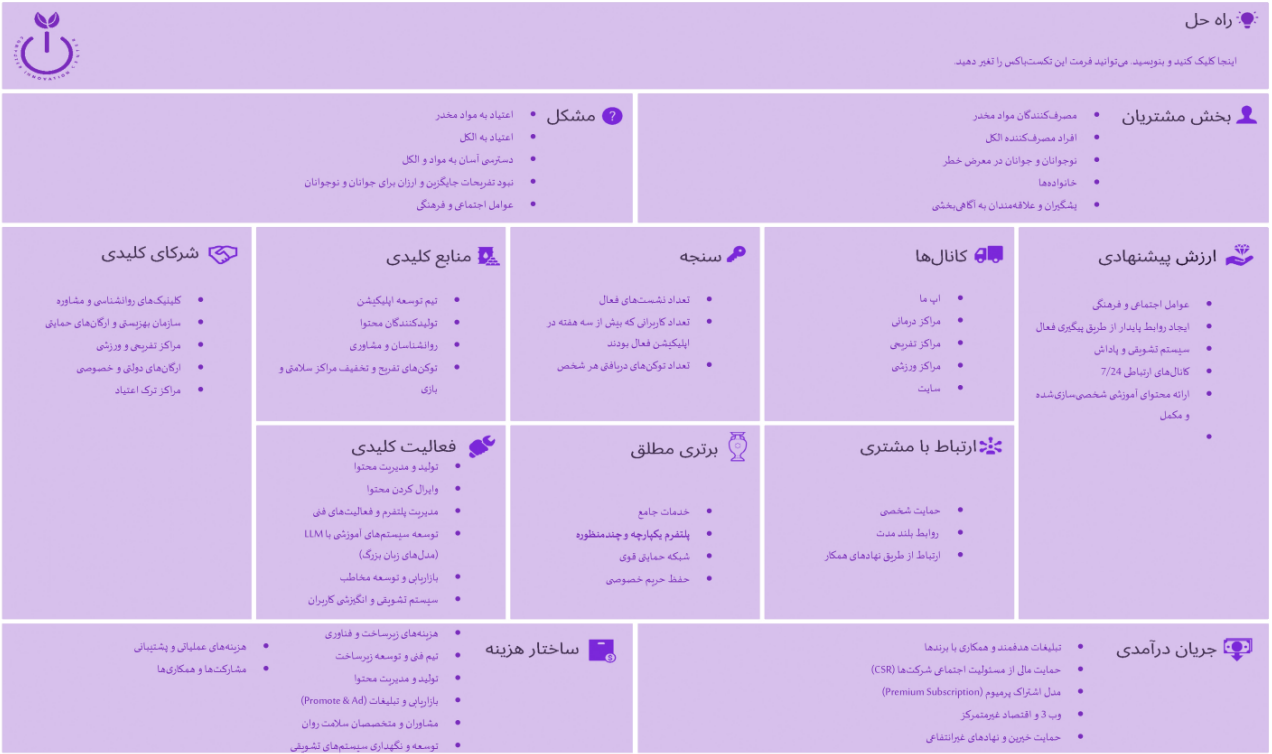
\includegraphics[scale=0.7, angle=90]{images/canvas1}
\end{center}
\caption{بوم کسب و کار}
\label{fig:lean-canvas}
\end{figure}


\begin{figure}[b]
\begin{center}
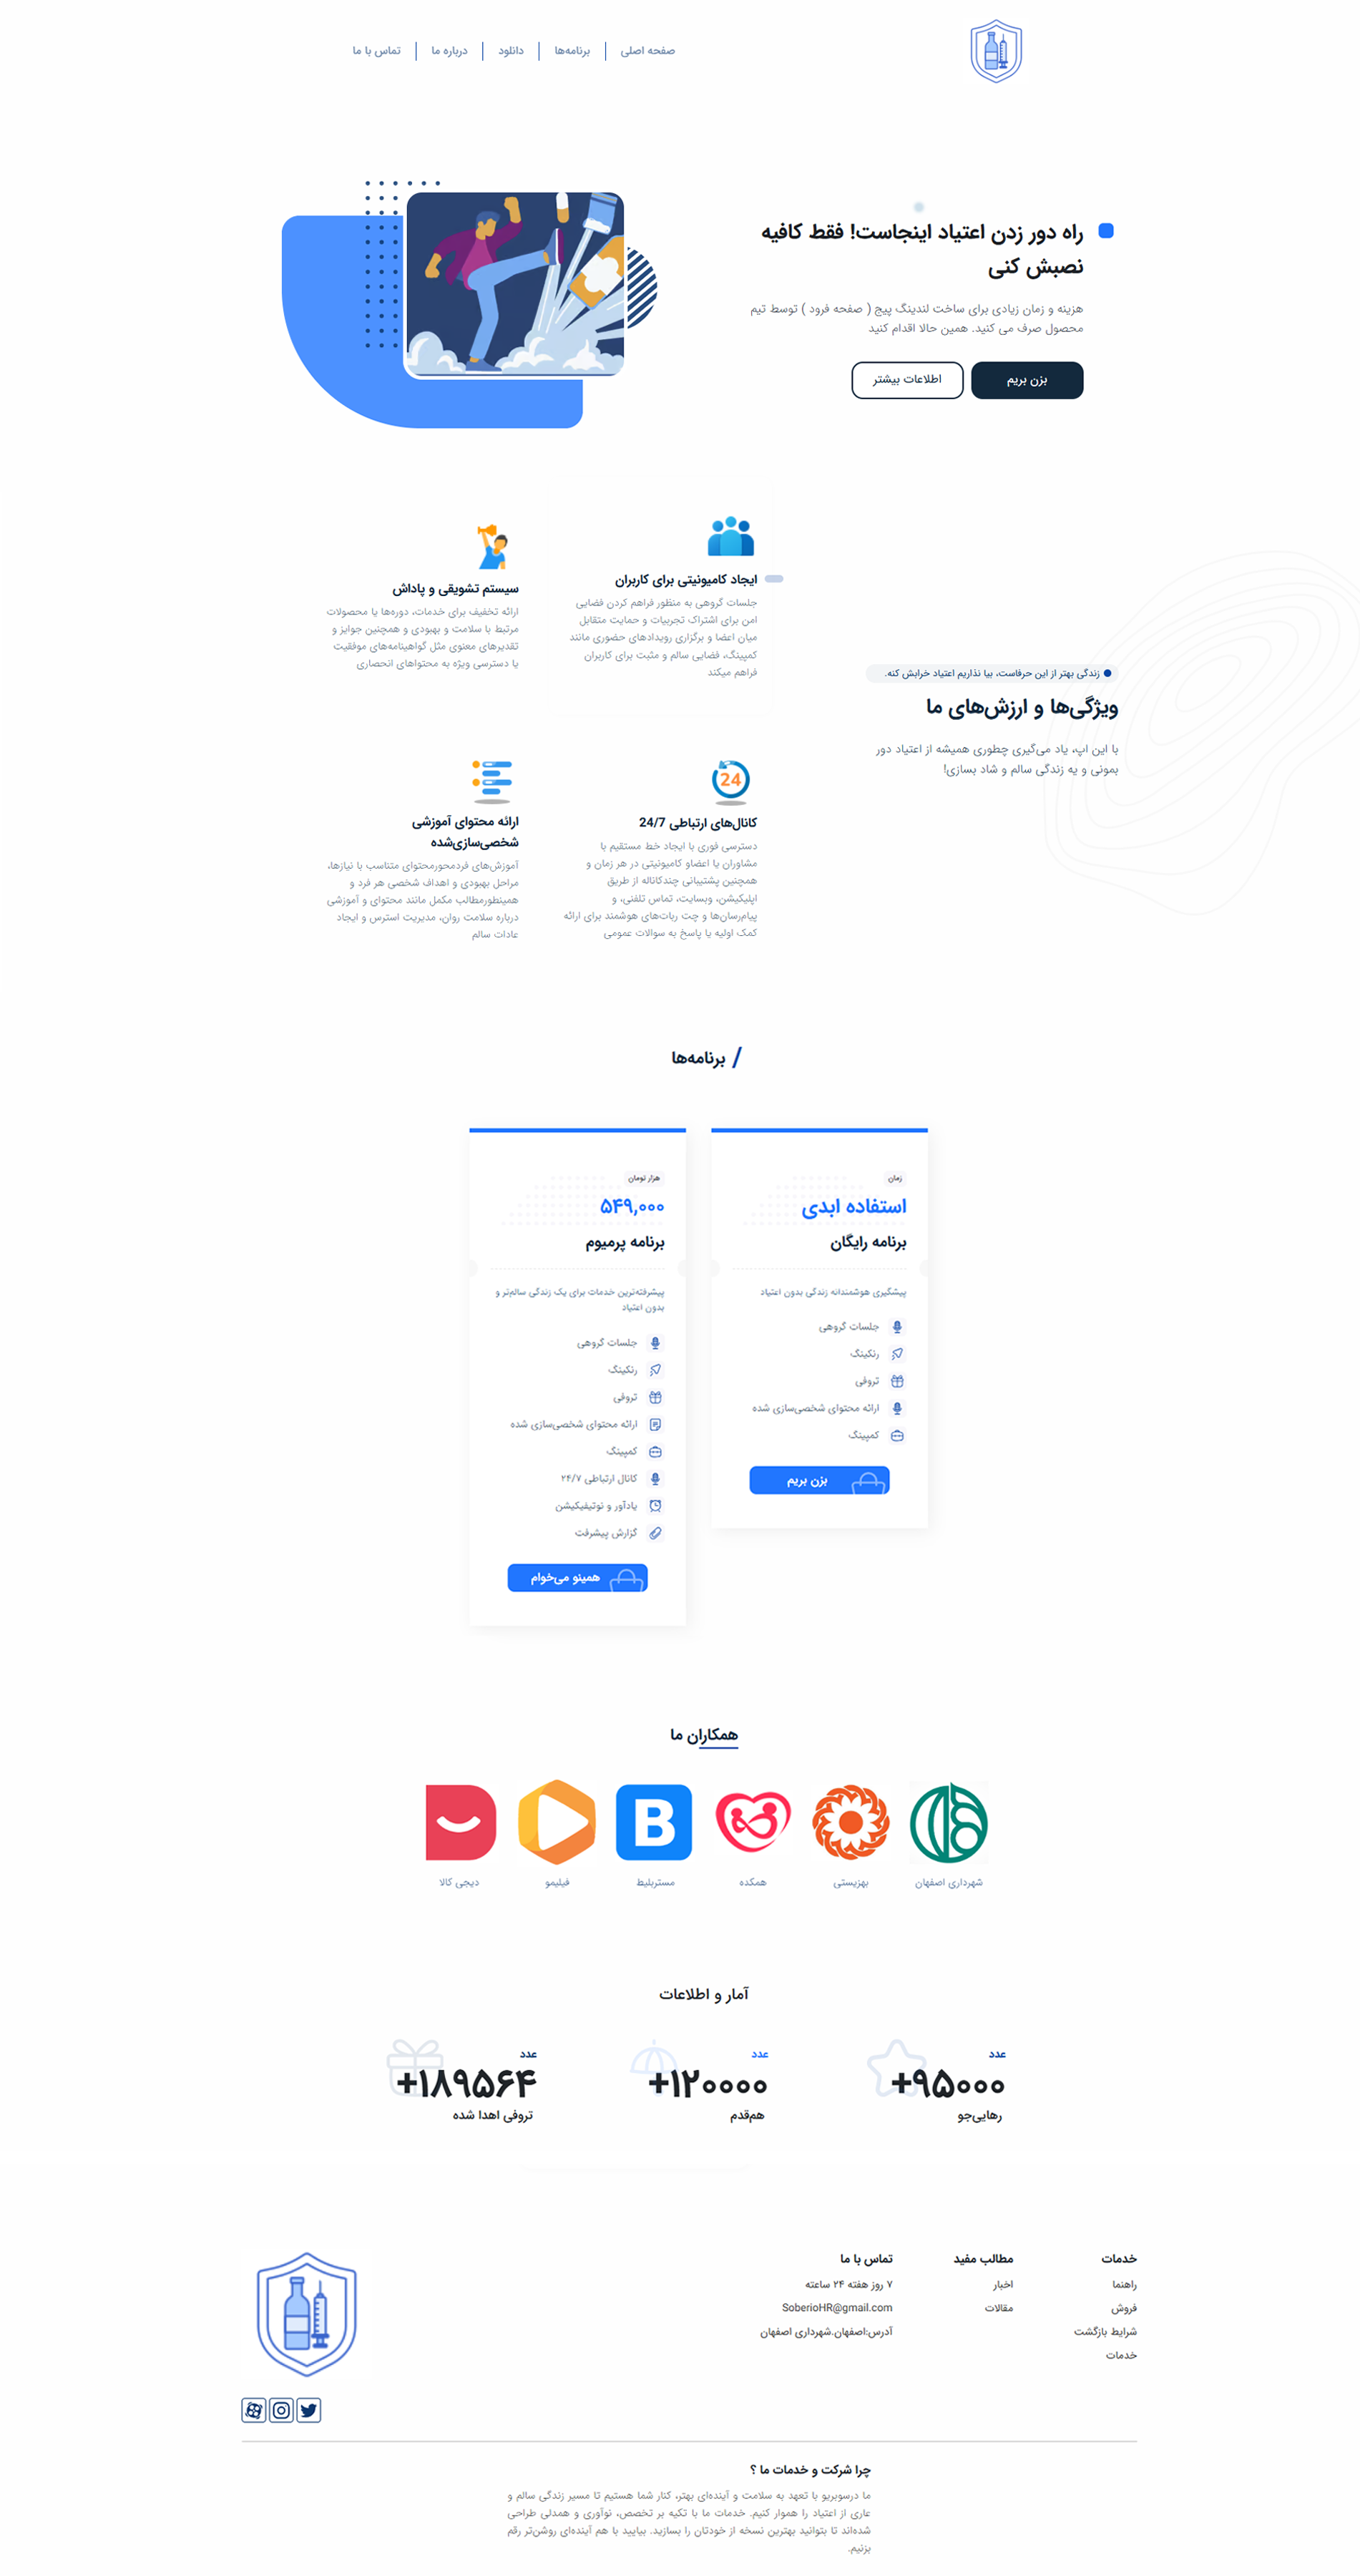
\includegraphics[scale=0.2]{images/landing}
\end{center}
\caption{لندینگ پیج}
\label{fig:landing-page}
\end{figure}

\end{document}